\usetikzlibrary{positioning, arrows.meta, shapes.geometric, patterns}

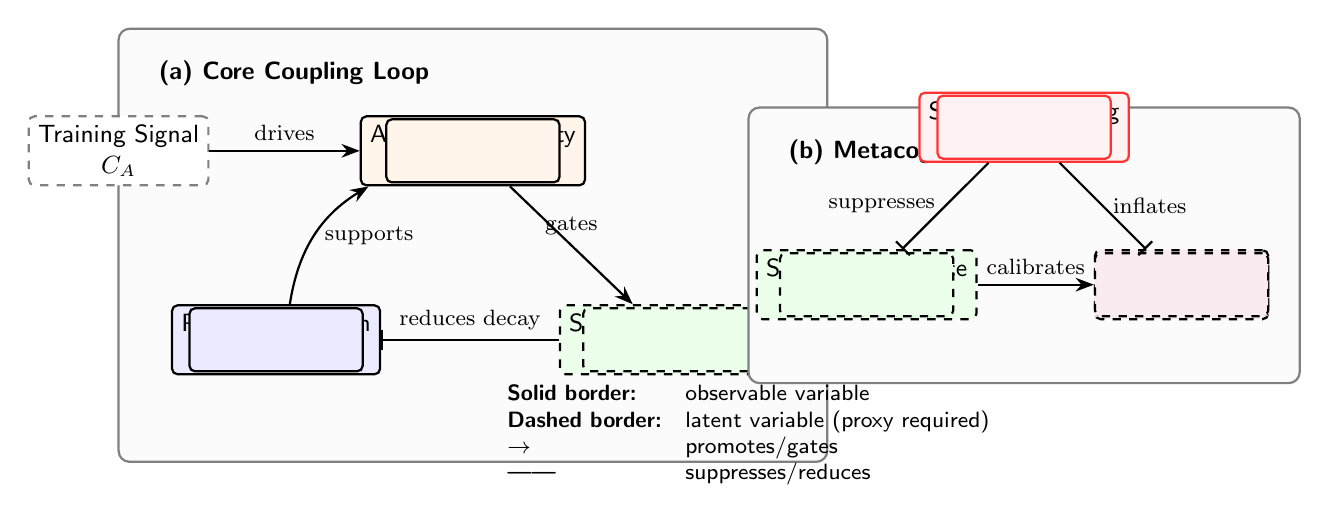
\begin{tikzpicture}[
    font=\sffamily,
    >=Stealth,
    node distance=1.8cm and 2.2cm,
    varbox/.style={rectangle, draw=black, thick, fill=white, rounded corners=2pt, minimum width=2.2cm, minimum height=0.8cm, align=center, font=\small\sffamily},
    latentbox/.style={rectangle, draw=black, thick, dashed, fill=white, rounded corners=2pt, minimum width=2.2cm, minimum height=0.8cm, align=center, font=\small\sffamily},
    panel/.style={draw=gray, thick, rounded corners=4pt, fill=gray!3},
    pos_edge/.style={->, thick, black},
    neg_edge/.style={-{Bar[width=2.5mm]}, thick, black},
]

    % ===== PANEL A: Core Coupling Loop =====
    \node[panel, minimum width=9cm, minimum height=5.5cm] (panelA) at (0,0) {};
    \node[anchor=north west, font=\small\bfseries\sffamily] at ([xshift=4mm, yshift=-3mm]panelA.north west) {(a) Core Coupling Loop};

    % Nodes for Panel A (with patterns for grayscale distinction)
    \node[varbox, fill=blue!8] (deltaA) at (-2.5,-1.2) {Parametric Depth\\$\delta_A$};
    \fill[pattern=north west lines, pattern color=blue!30] (-2.5-1.1,-1.2-0.4) rectangle (-2.5+1.1,-1.2+0.4);
    \node[latentbox, fill=green!8] (sigmaA) at (2.5,-1.2) {Schema Coherence\\$\sigma_A$};
    \fill[pattern=dots, pattern color=green!40] (2.5-1.1,-1.2-0.4) rectangle (2.5+1.1,-1.2+0.4);
    \node[varbox, fill=orange!8] (alphaA) at (0,1.2) {Attentional Fidelity\\$\alpha_A$};
    \fill[pattern=crosshatch, pattern color=orange!40] (0-1.1,1.2-0.4) rectangle (0+1.1,1.2+0.4);
    \node[varbox, draw=gray, dashed] (CA) at (-4.5,1.2) {Training Signal\\$C_A$};

    % Re-draw node borders on top of patterns
    \node[varbox, fill=blue!8, draw=black] (deltaA2) at (-2.5,-1.2) {};
    \node[latentbox, fill=green!8, draw=black] (sigmaA2) at (2.5,-1.2) {};
    \node[varbox, fill=orange!8, draw=black] (alphaA2) at (0,1.2) {};

    % Edges for Panel A
    \draw[pos_edge] (CA) -- node[above, font=\footnotesize] {drives} (alphaA);
    \draw[pos_edge] (alphaA) -- node[above, font=\footnotesize] {gates} (sigmaA);
    \draw[neg_edge] (sigmaA) -- node[above, font=\footnotesize] {reduces decay} (deltaA);
    \draw[pos_edge] (deltaA) to[bend left=25] node[right, font=\footnotesize] {supports} (alphaA);

    % ===== PANEL B: Metacognitive Extension =====
    \node[panel, minimum width=7cm, minimum height=3.5cm] (panelB) at (7,0) {};
    \node[anchor=north west, font=\small\bfseries\sffamily] at ([xshift=4mm, yshift=-3mm]panelB.north west) {(b) Metacognitive Extension};

    % Nodes for Panel B (with patterns)
    \node[latentbox, fill=green!8] (sigmaB) at (5,-0.5) {Schema Coherence\\$\sigma_A$};
    \fill[pattern=dots, pattern color=green!40] (5-1.1,-0.5-0.4) rectangle (5+1.1,-0.5+0.4);
    \node[latentbox, fill=purple!8] (MA) at (9,-0.5) {Self-Model\\$\hat{M}_A$};
    \fill[pattern=horizontal lines, pattern color=purple!30] (9-1.1,-0.5-0.4) rectangle (9+1.1,-0.5+0.4);
    \node[varbox, draw=red!80, fill=red!5] (Omega) at (7,1.5) {Shortcut Learning\\$\Omega_{SL}$};
    \fill[pattern=vertical lines, pattern color=red!30] (7-1.1,1.5-0.4) rectangle (7+1.1,1.5+0.4);

    % Re-draw borders on top
    \node[latentbox, fill=green!8, draw=black] (sigmaB2) at (5,-0.5) {};
    \node[latentbox, fill=purple!8, draw=black] (MA2) at (9,-0.5) {};
    \node[varbox, draw=red!80, fill=red!5] (Omega2) at (7,1.5) {};

    % Edges for Panel B
    \draw[pos_edge] (sigmaB) -- node[above, font=\footnotesize] {calibrates} (MA);
    \draw[neg_edge] (Omega) -- node[right, font=\footnotesize] {inflates} (MA);
    \draw[neg_edge] (Omega) -- node[left, font=\footnotesize] {suppresses} (sigmaB);

    % ===== LEGEND =====
    \node[anchor=south, font=\footnotesize\sffamily] at (3.5,-3.2) {
        \begin{tabular}{l@{\quad}l}
            \textbf{Solid border:} & observable variable \\
            \textbf{Dashed border:} & latent variable (proxy required) \\
            \textbf{$\rightarrow$} & promotes/gates \\
            \textbf{---|} & suppresses/reduces \\
        \end{tabular}
    };

\end{tikzpicture}
